\documentclass[11pt]{beamer}
\usepackage{verbatim}
\usepackage{amsmath}
\usepackage{amsthm}
\usepackage{graphics}
\usepackage{color}
\usepackage{stmaryrd}\usefonttheme[onlymath]{serif}

\title{On Multiphase-Linear Ranking Functions}
\date{\today}
\author{Xie Li}

\begin{document}
\maketitle

\begin{frame}\frametitle{Motzkin's Transposition Theorem}
\begin{theorem}[Motzkin's Transposition Theorem]
For $A\in \mathbb{K}^{m\times n}, C\in \mathbb{K}^{l\times n}, b\in \mathbb{K}^m, $ and $d\in \mathbb{K}^l$. The formulae below are equivalent.
\begin{itemize}
\item $\forall x \in \mathbb{K}^n. \neg (Ax\le b \wedge Cx < d)$

\item $\exists \lambda \in \mathbb{K}^m. \exists \mu \in \mathbb{K}^l.$

$\lambda \ge 0 \wedge \mu \ge 0$

$\wedge \lambda^{T}A + \mu^TC = 0 \wedge \lambda^{T}b + \mu^Td \le 0 $

$\wedge (\lambda^Tb < 0 \vee \mu \ne 0)$

\end{itemize}
\end{theorem}


Intuition of Motzkin's transposition theorem:...
\end{frame}


\begin{frame}
\begin{lemma}[0]
Given an non-empty polyhedron $\mathcal{P}$ and linear functions $f_1, \ldots , f_k$ such that 

\begin{enumerate}
\item $\textbf{x}\in \mathcal{P}\rightarrow f_1(  \textbf{x}) > 0 \vee \ldots \wedge f_{k-1}(\textbf{x}) > 0 \vee f_{k}(\textbf{x}) \ge 0$

\item $\textbf{x} \in \mathcal{P} \not\rightarrow f_1(\textbf{x}) > 0 \vee \ldots f_{k-1}(\textbf{x}) > 0$

\end{enumerate}
There exists a non-negative constants $\mu_1, \ldots, \mu_{k-1}$ such that 

\[\textbf{x}\in \mathcal{P} \rightarrow \mu_1f_1(\textbf{x}) + \mu_{k-1}f_{k-1}(\textbf{x}) + f_k(\textbf{x}) \ge 0\]
\end{lemma}


\end{frame}

\begin{frame}\frametitle{LRF, Nested r.f. and M$\Phi$RF}



\end{frame}

\begin{frame}\frametitle{M$\Phi$RF to Nested r.f.}
\begin{theorem}[1]
If $\mathcal{Q}$ has a M$\Phi$RF of depth $d$, then it has a nested ranking function of depth at most $d$.


\end{theorem}

\begin{proof}
By induction on the depth $d$.
\begin{itemize}
\item $d = 1$: M$\Phi$RF and nested r.f. are both LRF.
\item $d > 1$: $d = 2$ e.g.
$\langle f_1, f_2\rangle$. When index $i = 1$, we do not impose bound on $f_2(\textbf{x})$. However, a bound is needed for $f_2'(\textbf{x}s)$ in nested r.f. $\langle f_1', f_2'\rangle$.

To solve the problem that $f_2(\textbf{x})$ might goes under $0$, when $\textbf{x}''$ is ranked by $f_1$. Consider  $\mathcal{Q}' = \mathcal{Q}\cap \{\textbf{x}''\in \mathbb{Q}^{2n}\mid f_1(\textbf{x}'') \le 0\}$


\end{itemize}


\end{proof}

\end{frame}

\begin{frame}\frametitle{M$\Phi$RF to Nested r.f.}
\begin{lemma}[1]
Let $\tau = \langle f_1, \ldots, f_d \rangle$ be an irredundant M$\Phi$RF for $\mathcal{Q}$, such that $\langle f_2, \ldots, f_d\rangle$ is a nested ranking function for $\mathcal{Q}' = \mathcal{Q}\cap \{\textbf{x}''\in \mathbb{Q}^{2n}\mid f_1(\textbf{x}) \le 0\}$. Then there is a nested ranking function of depth $d$ for $\mathcal{Q}$.

\end{lemma}
Prove by construction: construct a nested r.f. $\langle f_1', \ldots, f_d'\rangle$
\begin{center}
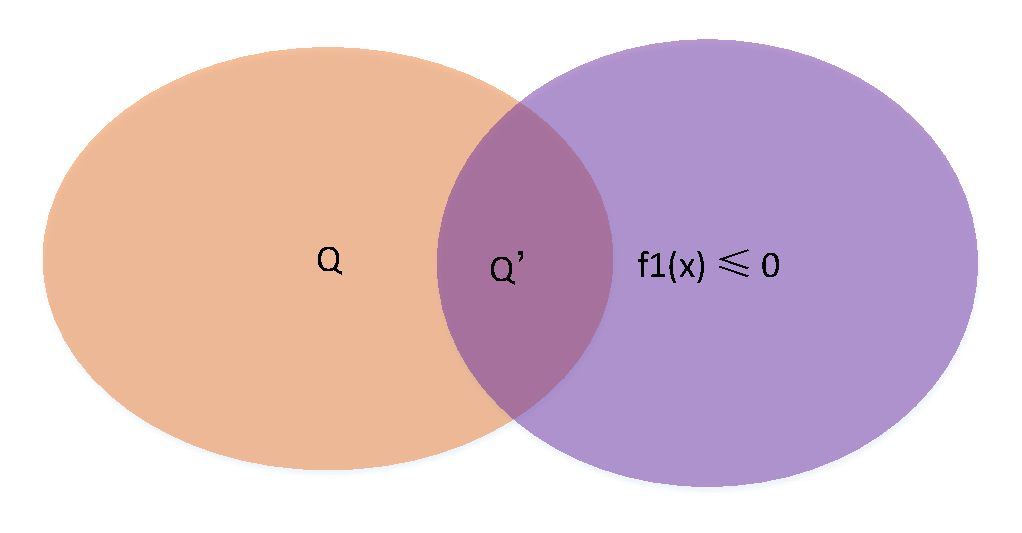
\includegraphics[scale = 0.3]{1.pdf}
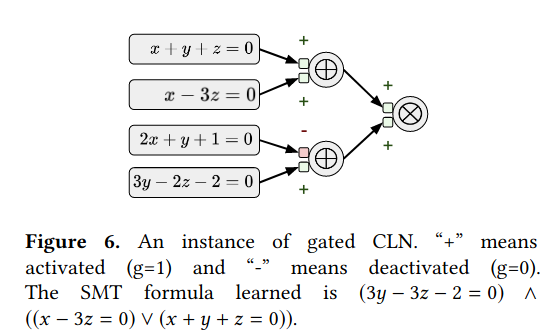
\includegraphics[scale = 0.2]{6.png}


\end{center}
If $f_d$ is non-negative on $\mathcal{Q}$, then $f_d' = f_d$.
Otherwise, $\textbf{x}'' \in \mathcal{Q} \rightarrow f_d(\textbf{x}) \ge 0 \vee f_1(\textbf{x}) > 0$


\end{frame}


\begin{frame}\frametitle{M$\Phi$RF to Nested r.f.}
\begin{center}
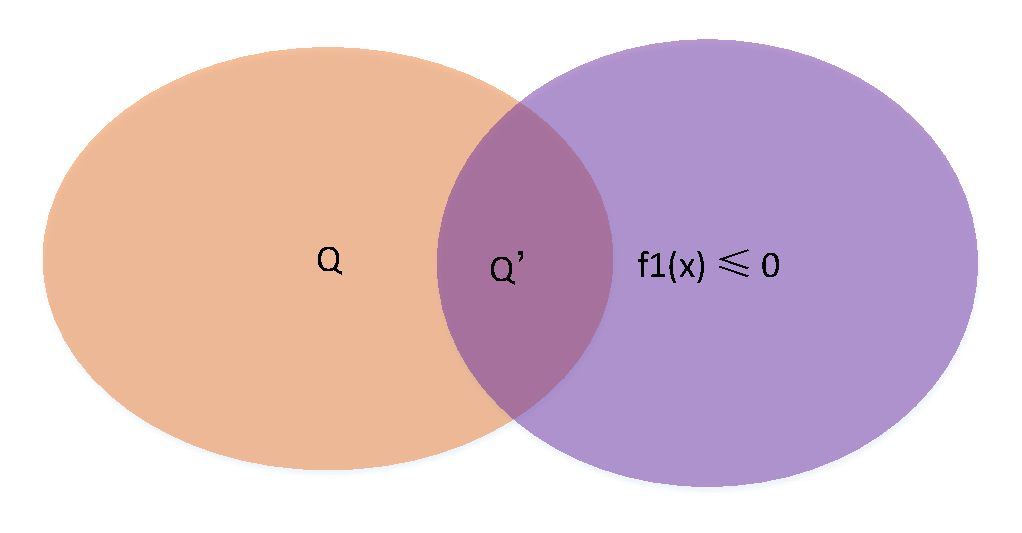
\includegraphics[scale = 0.3]{1.pdf}
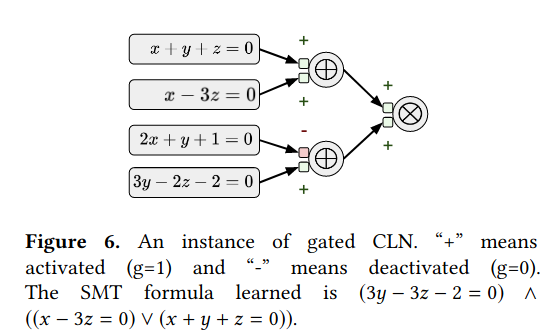
\includegraphics[scale = 0.2]{6.png}
\end{center}

Assume $f_{n}'(\textbf{x})= f_{n}(\textbf{x}) + \mu_{n}f_1(\textbf{x})$ and $f_d', \ldots, f_{i}'$ has already been computed.
\[\textbf{x}''\in \mathcal{Q}' \rightarrow (\Delta f_i(\textbf{x}'') - 1) + f_{i-1}(\textbf{x}) \ge 0\]
\[\textbf{x}''\in \mathcal{Q}' \rightarrow (\Delta f_i'(\textbf{x}'') - 1) + f_{i-1}(\textbf{x}) \ge 0\]
If above inequation also holds for $\mathcal{Q}$, then $f_{i-1}' = f_{i-1}$, Otherwise
\[\textbf{x}''\in \mathcal{Q} \rightarrow (\Delta f_i'(\textbf{x}'') - 1) + f_{i-1}(\textbf{x}) \ge 0 \vee f_1(\textbf{x}) \ge 0\]


\end{frame}

\begin{frame}\frametitle{BM$\Phi$RF($\mathbb{Q})\in$\texttt{PTIME}}
\begin{theorem}[2]
BM$\Phi$RF($\mathbb{Q}$)$\in$\texttt{PTIME}.



\end{theorem}

\begin{proof}


\end{proof}
\end{frame}


\begin{frame}\frametitle{LLRF}



\end{frame}

\begin{frame}\frametitle{Weak LLRF to M$\Phi$RF}

\begin{theorem}[3]
If $\mathcal{Q}$ has a weak LLRF of depth $d$, it has a  M$\Phi$RF of depth $d$.


\end{theorem}

\begin{proof}
Prove by induction.

\begin{itemize}

\item $d = 1$: 
For LLRF: $\Delta f_1(\textbf{x}'') > 0$, $f_1(\textbf{x}) \ge 0$ is a LRF due to the loop is linear.

For M$\Phi$RF: is a LRF.

\item $d > 1$: Observe that for a given LLRF $\langle f_1, f_2, \ldots, f_d\rangle $, after removing $f_k$, $\langle f_1, \ldots, f_{k-1}, f_{k+1}, \ldots, f_d\rangle$ is also a LLRF.

If we apply IH here, we get a M$\Phi$RF of depth $d-1$.

\end{itemize}


\end{proof}


\end{frame}


\begin{frame}\frametitle{Weak LLRF to M$\Phi$RF}
Now we want some techniques to use a M$\Phi$RF of depth $d-1$ and $f_k$ we removed to prove there is a M$\Phi$RF of depth $d$ on $\mathcal{Q}$. 
\begin{lemma}[2]
Let $f$ be a non-negative linear function over $\mathcal{Q}$. If $\mathcal{Q}' = \mathcal{Q}\ cap \{\textbf{x} '' \mid \Delta f(\textbf{x} '') \le 0\}$ has 

\end{lemma}


\end{frame}

\end{document}